% Options for packages loaded elsewhere
\PassOptionsToPackage{unicode}{hyperref}
\PassOptionsToPackage{hyphens}{url}
%
\documentclass[
]{article}
\usepackage{lmodern}
\usepackage{amssymb,amsmath}
\usepackage{ifxetex,ifluatex}
\ifnum 0\ifxetex 1\fi\ifluatex 1\fi=0 % if pdftex
  \usepackage[T1]{fontenc}
  \usepackage[utf8]{inputenc}
  \usepackage{textcomp} % provide euro and other symbols
\else % if luatex or xetex
  \usepackage{unicode-math}
  \defaultfontfeatures{Scale=MatchLowercase}
  \defaultfontfeatures[\rmfamily]{Ligatures=TeX,Scale=1}
\fi
% Use upquote if available, for straight quotes in verbatim environments
\IfFileExists{upquote.sty}{\usepackage{upquote}}{}
\IfFileExists{microtype.sty}{% use microtype if available
  \usepackage[]{microtype}
  \UseMicrotypeSet[protrusion]{basicmath} % disable protrusion for tt fonts
}{}
\makeatletter
\@ifundefined{KOMAClassName}{% if non-KOMA class
  \IfFileExists{parskip.sty}{%
    \usepackage{parskip}
  }{% else
    \setlength{\parindent}{0pt}
    \setlength{\parskip}{6pt plus 2pt minus 1pt}}
}{% if KOMA class
  \KOMAoptions{parskip=half}}
\makeatother
\usepackage{xcolor}
\IfFileExists{xurl.sty}{\usepackage{xurl}}{} % add URL line breaks if available
\IfFileExists{bookmark.sty}{\usepackage{bookmark}}{\usepackage{hyperref}}
\hypersetup{
  pdftitle={Lecture 2: Exploratory Data Analysis},
  pdfauthor={Xiao Guo},
  hidelinks,
  pdfcreator={LaTeX via pandoc}}
\urlstyle{same} % disable monospaced font for URLs
\usepackage[margin=1in]{geometry}
\usepackage{color}
\usepackage{fancyvrb}
\newcommand{\VerbBar}{|}
\newcommand{\VERB}{\Verb[commandchars=\\\{\}]}
\DefineVerbatimEnvironment{Highlighting}{Verbatim}{commandchars=\\\{\}}
% Add ',fontsize=\small' for more characters per line
\usepackage{framed}
\definecolor{shadecolor}{RGB}{248,248,248}
\newenvironment{Shaded}{\begin{snugshade}}{\end{snugshade}}
\newcommand{\AlertTok}[1]{\textcolor[rgb]{0.94,0.16,0.16}{#1}}
\newcommand{\AnnotationTok}[1]{\textcolor[rgb]{0.56,0.35,0.01}{\textbf{\textit{#1}}}}
\newcommand{\AttributeTok}[1]{\textcolor[rgb]{0.77,0.63,0.00}{#1}}
\newcommand{\BaseNTok}[1]{\textcolor[rgb]{0.00,0.00,0.81}{#1}}
\newcommand{\BuiltInTok}[1]{#1}
\newcommand{\CharTok}[1]{\textcolor[rgb]{0.31,0.60,0.02}{#1}}
\newcommand{\CommentTok}[1]{\textcolor[rgb]{0.56,0.35,0.01}{\textit{#1}}}
\newcommand{\CommentVarTok}[1]{\textcolor[rgb]{0.56,0.35,0.01}{\textbf{\textit{#1}}}}
\newcommand{\ConstantTok}[1]{\textcolor[rgb]{0.00,0.00,0.00}{#1}}
\newcommand{\ControlFlowTok}[1]{\textcolor[rgb]{0.13,0.29,0.53}{\textbf{#1}}}
\newcommand{\DataTypeTok}[1]{\textcolor[rgb]{0.13,0.29,0.53}{#1}}
\newcommand{\DecValTok}[1]{\textcolor[rgb]{0.00,0.00,0.81}{#1}}
\newcommand{\DocumentationTok}[1]{\textcolor[rgb]{0.56,0.35,0.01}{\textbf{\textit{#1}}}}
\newcommand{\ErrorTok}[1]{\textcolor[rgb]{0.64,0.00,0.00}{\textbf{#1}}}
\newcommand{\ExtensionTok}[1]{#1}
\newcommand{\FloatTok}[1]{\textcolor[rgb]{0.00,0.00,0.81}{#1}}
\newcommand{\FunctionTok}[1]{\textcolor[rgb]{0.00,0.00,0.00}{#1}}
\newcommand{\ImportTok}[1]{#1}
\newcommand{\InformationTok}[1]{\textcolor[rgb]{0.56,0.35,0.01}{\textbf{\textit{#1}}}}
\newcommand{\KeywordTok}[1]{\textcolor[rgb]{0.13,0.29,0.53}{\textbf{#1}}}
\newcommand{\NormalTok}[1]{#1}
\newcommand{\OperatorTok}[1]{\textcolor[rgb]{0.81,0.36,0.00}{\textbf{#1}}}
\newcommand{\OtherTok}[1]{\textcolor[rgb]{0.56,0.35,0.01}{#1}}
\newcommand{\PreprocessorTok}[1]{\textcolor[rgb]{0.56,0.35,0.01}{\textit{#1}}}
\newcommand{\RegionMarkerTok}[1]{#1}
\newcommand{\SpecialCharTok}[1]{\textcolor[rgb]{0.00,0.00,0.00}{#1}}
\newcommand{\SpecialStringTok}[1]{\textcolor[rgb]{0.31,0.60,0.02}{#1}}
\newcommand{\StringTok}[1]{\textcolor[rgb]{0.31,0.60,0.02}{#1}}
\newcommand{\VariableTok}[1]{\textcolor[rgb]{0.00,0.00,0.00}{#1}}
\newcommand{\VerbatimStringTok}[1]{\textcolor[rgb]{0.31,0.60,0.02}{#1}}
\newcommand{\WarningTok}[1]{\textcolor[rgb]{0.56,0.35,0.01}{\textbf{\textit{#1}}}}
\usepackage{graphicx,grffile}
\makeatletter
\def\maxwidth{\ifdim\Gin@nat@width>\linewidth\linewidth\else\Gin@nat@width\fi}
\def\maxheight{\ifdim\Gin@nat@height>\textheight\textheight\else\Gin@nat@height\fi}
\makeatother
% Scale images if necessary, so that they will not overflow the page
% margins by default, and it is still possible to overwrite the defaults
% using explicit options in \includegraphics[width, height, ...]{}
\setkeys{Gin}{width=\maxwidth,height=\maxheight,keepaspectratio}
% Set default figure placement to htbp
\makeatletter
\def\fps@figure{htbp}
\makeatother
\setlength{\emergencystretch}{3em} % prevent overfull lines
\providecommand{\tightlist}{%
  \setlength{\itemsep}{0pt}\setlength{\parskip}{0pt}}
\setcounter{secnumdepth}{-\maxdimen} % remove section numbering

\title{Lecture 2: Exploratory Data Analysis}
\author{Xiao Guo}
\date{2023/2/21}

\begin{document}
\maketitle

\hypertarget{exploratory-data-analysis}{%
\subsection{2.1. Exploratory Data
Analysis}\label{exploratory-data-analysis}}

\hypertarget{roles-of-data-visualization}{%
\subsubsection{Roles of Data
Visualization}\label{roles-of-data-visualization}}

\begin{itemize}
\tightlist
\item
  Role 1: Exploratory data analysis (pre stage);
\item
  Role 2: Visual presentation of results (after stage).
\item
  John W. Tukey (1977; Exploratory Data Analysis): ``The greatest value
  of a picture is when it forces us to notice what we never expected to
  see.''
\end{itemize}

\begin{Shaded}
\begin{Highlighting}[]
\NormalTok{knitr}\OperatorTok{::}\KeywordTok{include_graphics}\NormalTok{(}\StringTok{"tukey.png"}\NormalTok{)}
\end{Highlighting}
\end{Shaded}

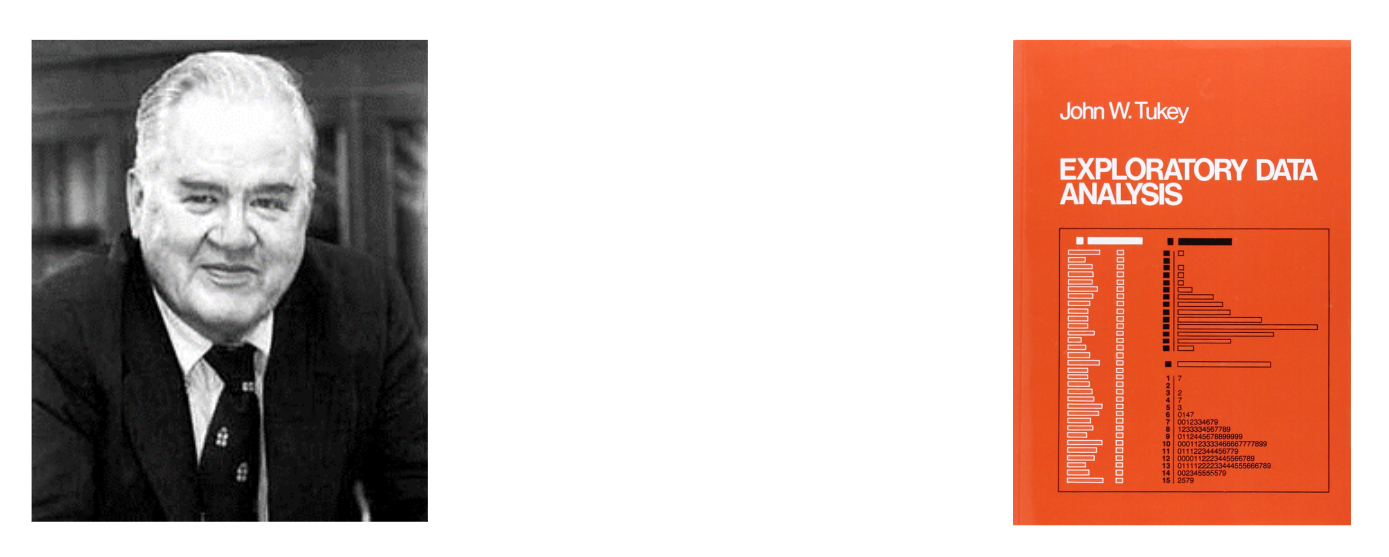
\includegraphics{tukey.png}

\hypertarget{john-tukey-1915-2000}{%
\subsubsection{John Tukey (1915-2000)}\label{john-tukey-1915-2000}}

Proposed ``Exploratory Data Analysis''

\begin{itemize}
\item
  Coined terms: Boxplot, Stem-and-Leaf plot, ANOVA (Analysis of
  Variance)
\item
  Coined terms ``Bit'' and ``Software''
\item
  Co-Developed Fast Fourier Transform algorithm, Projection Pursuit,
  Jackknife estimation
\item
  Famous quote: ``The best thing about being a statistician is that you
  get to play in everyone's backyard.''
\item
  \url{https://en.wikipedia.org/wiki/John_Tukey}
\end{itemize}

\hypertarget{john-tukey-exploratory-data-analysis-1977}{%
\subsubsection{John Tukey: Exploratory Data Analysis
(1977)}\label{john-tukey-exploratory-data-analysis-1977}}

\begin{itemize}
\item
  Five-number summary
\item
  Stem-and-Leaf plot
\item
  Scatter plot
\item
  Box-plot, Outliers
\item
  Residual plot
\item
  Smoother
\item
  Bag plot (two or three dimensional `box' plot)
\end{itemize}

\hypertarget{simple-base-graphics}{%
\subsection{2.2. Simple Base Graphics}\label{simple-base-graphics}}

\hypertarget{iris-dataset}{%
\subsubsection{Iris Dataset}\label{iris-dataset}}

\begin{Shaded}
\begin{Highlighting}[]
\NormalTok{DataX =}\StringTok{ }\NormalTok{iris  }
\KeywordTok{str}\NormalTok{(DataX)}
\end{Highlighting}
\end{Shaded}

\begin{verbatim}
## 'data.frame':    150 obs. of  5 variables:
##  $ Sepal.Length: num  5.1 4.9 4.7 4.6 5 5.4 4.6 5 4.4 4.9 ...
##  $ Sepal.Width : num  3.5 3 3.2 3.1 3.6 3.9 3.4 3.4 2.9 3.1 ...
##  $ Petal.Length: num  1.4 1.4 1.3 1.5 1.4 1.7 1.4 1.5 1.4 1.5 ...
##  $ Petal.Width : num  0.2 0.2 0.2 0.2 0.2 0.4 0.3 0.2 0.2 0.1 ...
##  $ Species     : Factor w/ 3 levels "setosa","versicolor",..: 1 1 1 1 1 1 1 1 1 1 ...
\end{verbatim}

\begin{Shaded}
\begin{Highlighting}[]
\CommentTok{#DataX$Species}
\KeywordTok{dim}\NormalTok{(DataX)}
\end{Highlighting}
\end{Shaded}

\begin{verbatim}
## [1] 150   5
\end{verbatim}

\begin{Shaded}
\begin{Highlighting}[]
\KeywordTok{head}\NormalTok{(DataX)}
\end{Highlighting}
\end{Shaded}

\begin{verbatim}
##   Sepal.Length Sepal.Width Petal.Length Petal.Width Species
## 1          5.1         3.5          1.4         0.2  setosa
## 2          4.9         3.0          1.4         0.2  setosa
## 3          4.7         3.2          1.3         0.2  setosa
## 4          4.6         3.1          1.5         0.2  setosa
## 5          5.0         3.6          1.4         0.2  setosa
## 6          5.4         3.9          1.7         0.4  setosa
\end{verbatim}

\begin{Shaded}
\begin{Highlighting}[]
\KeywordTok{summary}\NormalTok{(DataX)}
\end{Highlighting}
\end{Shaded}

\begin{verbatim}
##   Sepal.Length    Sepal.Width     Petal.Length    Petal.Width   
##  Min.   :4.300   Min.   :2.000   Min.   :1.000   Min.   :0.100  
##  1st Qu.:5.100   1st Qu.:2.800   1st Qu.:1.600   1st Qu.:0.300  
##  Median :5.800   Median :3.000   Median :4.350   Median :1.300  
##  Mean   :5.843   Mean   :3.057   Mean   :3.758   Mean   :1.199  
##  3rd Qu.:6.400   3rd Qu.:3.300   3rd Qu.:5.100   3rd Qu.:1.800  
##  Max.   :7.900   Max.   :4.400   Max.   :6.900   Max.   :2.500  
##        Species  
##  setosa    :50  
##  versicolor:50  
##  virginica :50  
##                 
##                 
## 
\end{verbatim}

\hypertarget{basic-r-plots}{%
\subsubsection{Basic R Plots}\label{basic-r-plots}}

\hypertarget{histogram}{%
\paragraph{Histogram}\label{histogram}}

\begin{Shaded}
\begin{Highlighting}[]
\NormalTok{x =}\StringTok{ }\NormalTok{DataX[,}\DecValTok{1}\NormalTok{]}
\KeywordTok{hist}\NormalTok{(x, }\DataTypeTok{main=}\StringTok{'Histogram (Default)'}\NormalTok{)   }
\end{Highlighting}
\end{Shaded}

\includegraphics{Lecture-2_files/figure-latex/unnamed-chunk-3-1.pdf}

\begin{Shaded}
\begin{Highlighting}[]
\KeywordTok{hist}\NormalTok{(x, }\DataTypeTok{breaks=}\DecValTok{20}\NormalTok{, }\DataTypeTok{col=}\StringTok{"orange"}\NormalTok{, }\DataTypeTok{main=}\StringTok{'More Bins and Coloring'}\NormalTok{) }
\end{Highlighting}
\end{Shaded}

\includegraphics{Lecture-2_files/figure-latex/unnamed-chunk-3-2.pdf}

\begin{Shaded}
\begin{Highlighting}[]
\KeywordTok{hist}\NormalTok{(x, }\DataTypeTok{breaks=}\DecValTok{20}\NormalTok{, }\DataTypeTok{freq=}\NormalTok{F, }\DataTypeTok{main=}\StringTok{'Histogram plus Density Plot'}\NormalTok{)   }\CommentTok{# using freq=FALSE}
\KeywordTok{lines}\NormalTok{(}\KeywordTok{density}\NormalTok{(x), }\DataTypeTok{col=}\DecValTok{2}\NormalTok{, }\DataTypeTok{lty=}\DecValTok{1}\NormalTok{, }\DataTypeTok{lwd=}\DecValTok{2}\NormalTok{)  }\CommentTok{#add the density curve}
\end{Highlighting}
\end{Shaded}

\includegraphics{Lecture-2_files/figure-latex/unnamed-chunk-3-3.pdf}

\hypertarget{box-plot}{%
\paragraph{Box plot}\label{box-plot}}

\begin{Shaded}
\begin{Highlighting}[]
\NormalTok{x =}\StringTok{ }\NormalTok{DataX[,}\DecValTok{2}\NormalTok{]}
\KeywordTok{boxplot}\NormalTok{(x,}\DataTypeTok{main=}\StringTok{"Box plot"}\NormalTok{,}\DataTypeTok{col=}\StringTok{"gold"}\NormalTok{)}
\KeywordTok{mtext}\NormalTok{(}\StringTok{"Speal Width"}\NormalTok{, }\DataTypeTok{side =} \DecValTok{2}\NormalTok{, }\DataTypeTok{line =} \FloatTok{2.8}\NormalTok{,}\DataTypeTok{cex=}\FloatTok{1.4}\NormalTok{)}
\end{Highlighting}
\end{Shaded}

\includegraphics{Lecture-2_files/figure-latex/unnamed-chunk-4-1.pdf}

\begin{Shaded}
\begin{Highlighting}[]
\KeywordTok{boxplot}\NormalTok{(DataX[,}\DecValTok{1}\OperatorTok{:}\DecValTok{4}\NormalTok{], }\DataTypeTok{col=}\KeywordTok{c}\NormalTok{(}\DecValTok{2}\NormalTok{,}\DecValTok{3}\NormalTok{,}\DecValTok{4}\NormalTok{,}\DecValTok{5}\NormalTok{), }\DataTypeTok{main=}\StringTok{'Side-by-side Boxplot'}\NormalTok{) }
\end{Highlighting}
\end{Shaded}

\includegraphics{Lecture-2_files/figure-latex/unnamed-chunk-4-2.pdf}

\begin{Shaded}
\begin{Highlighting}[]
\KeywordTok{boxplot}\NormalTok{(Sepal.Length}\OperatorTok{~}\NormalTok{Species, DataX, }\DataTypeTok{col=}\KeywordTok{c}\NormalTok{(}\DecValTok{6}\NormalTok{,}\DecValTok{7}\NormalTok{,}\DecValTok{8}\NormalTok{), }\DataTypeTok{main=}\StringTok{"Boxplot with Grouping"}\NormalTok{)}
\end{Highlighting}
\end{Shaded}

\includegraphics{Lecture-2_files/figure-latex/unnamed-chunk-4-3.pdf}

\begin{Shaded}
\begin{Highlighting}[]
\KeywordTok{boxplot}\NormalTok{(Petal.Length}\OperatorTok{~}\NormalTok{Species, DataX, }\DataTypeTok{col=}\KeywordTok{c}\NormalTok{(}\DecValTok{6}\NormalTok{,}\DecValTok{7}\NormalTok{,}\DecValTok{8}\NormalTok{), }\DataTypeTok{main=}\StringTok{"Boxplot with Grouping"}\NormalTok{)}
\end{Highlighting}
\end{Shaded}

\includegraphics{Lecture-2_files/figure-latex/unnamed-chunk-4-4.pdf}

\begin{Shaded}
\begin{Highlighting}[]
\KeywordTok{boxplot}\NormalTok{(Sepal.Width}\OperatorTok{~}\NormalTok{Species, DataX, }\DataTypeTok{col=}\KeywordTok{c}\NormalTok{(}\DecValTok{6}\NormalTok{,}\DecValTok{7}\NormalTok{,}\DecValTok{8}\NormalTok{), }\DataTypeTok{main=}\StringTok{"Boxplot with Grouping"}\NormalTok{)}
\end{Highlighting}
\end{Shaded}

\includegraphics{Lecture-2_files/figure-latex/unnamed-chunk-4-5.pdf}

\begin{Shaded}
\begin{Highlighting}[]
\KeywordTok{boxplot}\NormalTok{(Petal.Width}\OperatorTok{~}\NormalTok{Species, DataX, }\DataTypeTok{col=}\KeywordTok{c}\NormalTok{(}\DecValTok{6}\NormalTok{,}\DecValTok{7}\NormalTok{,}\DecValTok{8}\NormalTok{), }\DataTypeTok{main=}\StringTok{"Boxplot with Grouping"}\NormalTok{)}
\end{Highlighting}
\end{Shaded}

\includegraphics{Lecture-2_files/figure-latex/unnamed-chunk-4-6.pdf}

\hypertarget{pie-and-bar-charts}{%
\paragraph{Pie and Bar Charts}\label{pie-and-bar-charts}}

\begin{Shaded}
\begin{Highlighting}[]
\NormalTok{DataX}\OperatorTok{$}\NormalTok{Flag =}\StringTok{ }\NormalTok{DataX}\OperatorTok{$}\NormalTok{Sepal.Length}\OperatorTok{>}\DecValTok{5} \CommentTok{# Create a binary flag}
\KeywordTok{pie}\NormalTok{(}\KeywordTok{table}\NormalTok{(DataX}\OperatorTok{$}\NormalTok{Species[DataX}\OperatorTok{$}\NormalTok{Flag]), }\DataTypeTok{col=}\KeywordTok{c}\NormalTok{(}\DecValTok{2}\NormalTok{,}\DecValTok{3}\NormalTok{,}\DecValTok{4}\NormalTok{))}
\end{Highlighting}
\end{Shaded}

\includegraphics{Lecture-2_files/figure-latex/unnamed-chunk-5-1.pdf}

\begin{Shaded}
\begin{Highlighting}[]
\KeywordTok{barplot}\NormalTok{(}\KeywordTok{table}\NormalTok{(DataX}\OperatorTok{$}\NormalTok{Species[DataX}\OperatorTok{$}\NormalTok{Flag]), }\DataTypeTok{col=}\KeywordTok{c}\NormalTok{(}\DecValTok{5}\NormalTok{,}\DecValTok{6}\NormalTok{,}\DecValTok{7}\NormalTok{))}
\end{Highlighting}
\end{Shaded}

\includegraphics{Lecture-2_files/figure-latex/unnamed-chunk-5-2.pdf}

\begin{Shaded}
\begin{Highlighting}[]
\KeywordTok{barplot}\NormalTok{(}\KeywordTok{table}\NormalTok{(DataX}\OperatorTok{$}\NormalTok{Species, DataX}\OperatorTok{$}\NormalTok{Flag), }\DataTypeTok{col=}\KeywordTok{c}\NormalTok{(}\DecValTok{5}\NormalTok{,}\DecValTok{6}\NormalTok{,}\DecValTok{7}\NormalTok{), }\DataTypeTok{beside=}\NormalTok{T)}
\end{Highlighting}
\end{Shaded}

\includegraphics{Lecture-2_files/figure-latex/unnamed-chunk-5-3.pdf}

\hypertarget{relationship-between-variables}{%
\paragraph{Relationship Between
Variables}\label{relationship-between-variables}}

\begin{Shaded}
\begin{Highlighting}[]
\NormalTok{x =}\StringTok{ }\NormalTok{DataX}\OperatorTok{$}\NormalTok{Petal.Length; y =}\StringTok{ }\NormalTok{DataX}\OperatorTok{$}\NormalTok{Petal.Width; z =}\StringTok{ }\NormalTok{DataX}\OperatorTok{$}\NormalTok{Species}
\KeywordTok{plot}\NormalTok{(x, y, }\DataTypeTok{xlab=}\StringTok{"Petal.Length"}\NormalTok{, }\DataTypeTok{ylab=}\StringTok{"Petal.Width"}\NormalTok{) }
\KeywordTok{abline}\NormalTok{(}\KeywordTok{coef}\NormalTok{(}\KeywordTok{lm}\NormalTok{(y}\OperatorTok{~}\NormalTok{x)), }\DataTypeTok{col=}\DecValTok{1}\NormalTok{, }\DataTypeTok{lty=}\DecValTok{2}\NormalTok{)}
\end{Highlighting}
\end{Shaded}

\includegraphics{Lecture-2_files/figure-latex/unnamed-chunk-6-1.pdf}

\begin{Shaded}
\begin{Highlighting}[]
\KeywordTok{plot}\NormalTok{(x, y, }\DataTypeTok{col=}\KeywordTok{c}\NormalTok{(}\DecValTok{2}\NormalTok{,}\DecValTok{3}\NormalTok{,}\DecValTok{4}\NormalTok{)[z], }\DataTypeTok{pch=}\DecValTok{20}\NormalTok{, }\DataTypeTok{cex=}\FloatTok{2.0}\NormalTok{, }\DataTypeTok{xlab=}\StringTok{"Petal.Length"}\NormalTok{, }\DataTypeTok{ylab=}\StringTok{"Petal.Width"}\NormalTok{) }
\KeywordTok{abline}\NormalTok{(}\KeywordTok{lm}\NormalTok{(y}\OperatorTok{~}\NormalTok{x), }\DataTypeTok{col=}\DecValTok{1}\NormalTok{, }\DataTypeTok{lty=}\DecValTok{2}\NormalTok{) }
\KeywordTok{legend}\NormalTok{(}\StringTok{"topleft"}\NormalTok{, }\KeywordTok{levels}\NormalTok{(z), }\DataTypeTok{pch=}\DecValTok{20}\NormalTok{, }\DataTypeTok{col=}\KeywordTok{c}\NormalTok{(}\DecValTok{2}\NormalTok{,}\DecValTok{3}\NormalTok{,}\DecValTok{4}\NormalTok{))}
\end{Highlighting}
\end{Shaded}

\includegraphics{Lecture-2_files/figure-latex/unnamed-chunk-6-2.pdf}

\hypertarget{pairwise-scatter-plot}{%
\paragraph{Pairwise Scatter Plot}\label{pairwise-scatter-plot}}

\begin{Shaded}
\begin{Highlighting}[]
\KeywordTok{plot}\NormalTok{(DataX, }\DataTypeTok{col=}\NormalTok{DataX}\OperatorTok{$}\NormalTok{Species, }\DataTypeTok{main=}\StringTok{"Pairwise Scatter Plot"}\NormalTok{)}
\end{Highlighting}
\end{Shaded}

\includegraphics{Lecture-2_files/figure-latex/unnamed-chunk-7-1.pdf}

\begin{Shaded}
\begin{Highlighting}[]
\KeywordTok{pairs}\NormalTok{(DataX[,}\DecValTok{1}\OperatorTok{:}\DecValTok{4}\NormalTok{], }\DataTypeTok{panel =}\NormalTok{ panel.smooth, }\DataTypeTok{col =} \KeywordTok{c}\NormalTok{(}\DecValTok{4}\NormalTok{,}\DecValTok{5}\NormalTok{,}\DecValTok{6}\NormalTok{)[DataX}\OperatorTok{$}\NormalTok{Species], }\DataTypeTok{main=}\StringTok{"More Sophisticated"}\NormalTok{)}
\end{Highlighting}
\end{Shaded}

\includegraphics{Lecture-2_files/figure-latex/unnamed-chunk-7-2.pdf}

\hypertarget{bag-plot}{%
\paragraph{Bag Plot}\label{bag-plot}}

\begin{itemize}
\item
  The bagplot consists of three nested polygons, called the ``bag'', the
  ``fence'', and the ``loop''.
\item
  The inner polygon, called the bag, is constructed on the basis of
  Tukey depth, the smallest number of observations that can be contained
  by a half-plane that also contains a given point.{[}4{]} It contains
  at most 50\% of the data points.
\item
  The outermost of the three polygons, called the fence is not drawn as
  part of the bagplot, but is used to construct it. It is formed by
  inflating the bag by a certain factor (usually 3). Observations
  outside the fence are flagged as outliers.
\item
  The observations that are not marked as outliers are surrounded by a
  loop, the convex hull of the observations within the fence.
\end{itemize}

\begin{Shaded}
\begin{Highlighting}[]
\KeywordTok{library}\NormalTok{(aplpack)}
\end{Highlighting}
\end{Shaded}

\begin{verbatim}
## Warning: package 'aplpack' was built under R version 4.0.5
\end{verbatim}

\begin{Shaded}
\begin{Highlighting}[]
\KeywordTok{bagplot}\NormalTok{(DataX[, }\DecValTok{1}\OperatorTok{:}\DecValTok{2}\NormalTok{])}
\end{Highlighting}
\end{Shaded}

\includegraphics{Lecture-2_files/figure-latex/unnamed-chunk-8-1.pdf}

\hypertarget{violin-plot}{%
\paragraph{Violin Plot}\label{violin-plot}}

A violin plot is a hybrid of a box plot and a kernel density plot, which
shows peaks in the data. It is used to visualize the distribution of
numerical data. Unlike a box plot that can only show summary statistics,
violin plots depict summary statistics and the density of each variable.

\begin{Shaded}
\begin{Highlighting}[]
\KeywordTok{library}\NormalTok{(vioplot)}
\end{Highlighting}
\end{Shaded}

\begin{verbatim}
## Loading required package: sm
\end{verbatim}

\begin{verbatim}
## Package 'sm', version 2.2-5.7: type help(sm) for summary information
\end{verbatim}

\begin{verbatim}
## Loading required package: zoo
\end{verbatim}

\begin{verbatim}
## 
## Attaching package: 'zoo'
\end{verbatim}

\begin{verbatim}
## The following objects are masked from 'package:base':
## 
##     as.Date, as.Date.numeric
\end{verbatim}

\begin{Shaded}
\begin{Highlighting}[]
\KeywordTok{vioplot}\NormalTok{(DataX[,}\DecValTok{1}\NormalTok{], DataX[,}\DecValTok{2}\NormalTok{],}\DataTypeTok{col=}\DecValTok{4}\NormalTok{)}
\end{Highlighting}
\end{Shaded}

\includegraphics{Lecture-2_files/figure-latex/unnamed-chunk-9-1.pdf}

\end{document}
